\tikzset{fontscale/.style = {font=\relsize{#1}}
    }
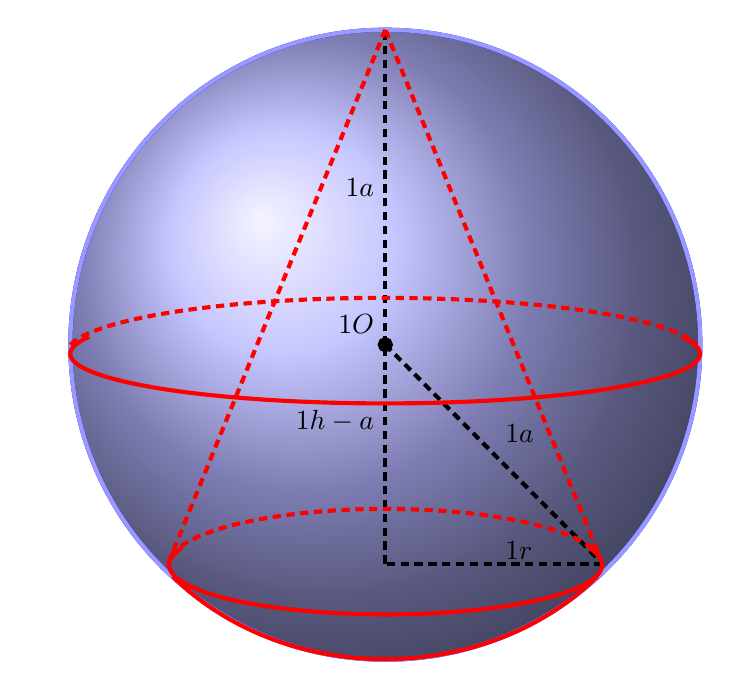
\begin{tikzpicture}[font = \sansmath,fontscale=1,scale=2,line width=1.5pt]
%\draw [very thin, style=gray!50, step=0.5] (-3,-2) grid (3,2);
  \coordinate (O) at (0,0);
 \coordinate (A) at (-1.38,1.39);
 \coordinate (B) at (-1.38,-1.39);
 \coordinate (C) at (1.38,1.39);
 \coordinate (D) at (1.38,-1.39);
\coordinate (E) at (0,-1.39);
\coordinate (F) at (0,2);



  % ball background color
 \shadedraw[shading=ball,ball color=blue!30, blue](0,0) circle [radius = 2cm];
  

  % ball
  \draw [blue!40](O) circle [radius=2cm];
  
  % radius
  \draw[densely dashed] (O) to [edge label = $a$] (D);
  \draw[densely dashed] (O)to [edge label = $a$]  (F);
% label of ball center point
  \filldraw (O) circle (1pt) node[above left] {$O$};

%cilindro
 \draw[densely dashed,red] (D) to (F);
\draw[densely dashed,red] (F) to (B);
\draw[densely dashed] (D) to [above=12pt,edge label = $r$] (E);
\draw[densely dashed] (E) to [above=12pt,edge label = $h-a$] (O);

  % cut of ball surface botton
  \draw[red] (-1.35,-1.47) arc [start angle = -140, end angle = -40,
    x radius = 17.6mm, y radius = 14.75mm];
  \draw[red, densely dashed] (-1.36,-1.34) arc [start angle = 170, end angle = 10,
    x radius = 13.8mm, y radius = 3.6mm];
  \draw[red] (-1.29,-1.29) arc [start angle=-200, end angle = 20,
    x radius = 13.75mm, y radius = 3.15mm];

%centro of ball 
 \draw[red, densely dashed] (-2,0) arc [start angle = 170, end angle = 10,
    x radius = 20.2mm, y radius = 3.6mm];
  \draw[red] (-1.88,0.05) arc [start angle=-200, end angle = 20,
    x radius = 20mm, y radius = 3.15mm];

\end{tikzpicture}
